\documentclass[11pt,a4paper]{article}
\usepackage[spanish,es-noshorthands,es-tabla]{babel}
\usepackage{analysis_orax}   % plantilla: fuente, colores, títulos, encabezado y pie
% La ola del pie mide 29 mm: el margen inferior se agranda para que el texto no la pise
\geometry{bottom=3.3cm,footskip=1.6cm}
\usepackage{graphicx,booktabs,tabularx,array,amsmath,amssymb,enumitem,float,caption,needspace,multirow}
\usepackage[most]{tcolorbox}
\usepackage{tikz}
\usetikzlibrary{arrows.meta,positioning,fit,calc,shapes.geometric,backgrounds}
\usepackage[hidelinks]{hyperref}
\usepackage{lastpage}

\graphicspath{{figures/}{../img/}{../plan/}}
\setmonofont{Fira Mono}[Scale=0.88]
\setlength{\headheight}{16pt}
\setlength{\parskip}{4pt}
\setlength{\parindent}{0pt}
\setlength{\emergencystretch}{3em}
\makeatletter\g@addto@macro\UrlBreaks{\do\_}\makeatother
\renewcommand{\arraystretch}{1.25}
\captionsetup{font=small,labelfont={bf,color=Orange},textfont={color=DarkGray}}
\setlist{itemsep=2pt,topsep=3pt}
\setcounter{tocdepth}{1}
\renewcommand{\topfraction}{0.85}\renewcommand{\bottomfraction}{0.6}\renewcommand{\textfraction}{0.12}\renewcommand{\floatpagefraction}{0.75}
\definecolor{Verde}{RGB}{46,125,50}
\definecolor{Rojo}{RGB}{198,40,40}
\definecolor{Gris}{RGB}{95,107,122}
\newcolumntype{Y}{>{\raggedright\arraybackslash}X}

% Recuadro de la plantilla de la skill: fondo de la hoja, barra lateral y título en acento
\newtcolorbox{destacado}[1][]{enhanced,breakable,colback=white,colframe=Orange,
  boxrule=0pt,leftrule=2.6pt,arc=0pt,outer arc=0pt,left=8pt,right=4pt,top=3pt,bottom=3pt,
  fonttitle=\bfseries\color{Orange},coltitle=Orange,colbacktitle=white,
  attach title to upper={\ },#1}
% Etiqueta de color para las etapas
\newcommand{\etapa}[2][DarkBlue]{\tikz[baseline=(t.base)]\node[fill=#1,text=white,font=\footnotesize\bfseries,
  rounded corners=2pt,inner sep=2.2pt](t){#2};}
\newcommand{\ok}{\textcolor{Verde}{$\checkmark$}}
\newcommand{\no}{\textcolor{Rojo}{$\times$}}
\newcommand{\seccion}[1]{\Needspace{18\baselineskip}\section{#1}}
\newcommand{\subsec}[1]{\Needspace{9\baselineskip}\subsection{#1}}

\begin{document}

%======================================================== PORTADA
\begin{titlepage}
\thispagestyle{fancy}
\vspace*{0.4cm}
{\color{Orange}\bfseries\large INFORME TÉCNICO · OPEN ROBOTICS 2026-2}\par
\vspace{0.5cm}
{\color{DarkBlue}\bfseries\fontsize{34}{38}\selectfont Hexápodo simulado\\[2pt] con ROS\,2}\par
\vspace{0.35cm}
{\color{MediumBlue}\Large Modelo, marcha trípode, sensores, micro-ROS\\ y estudio de dimensiones para el robot real}\par
\vspace{0.7cm}
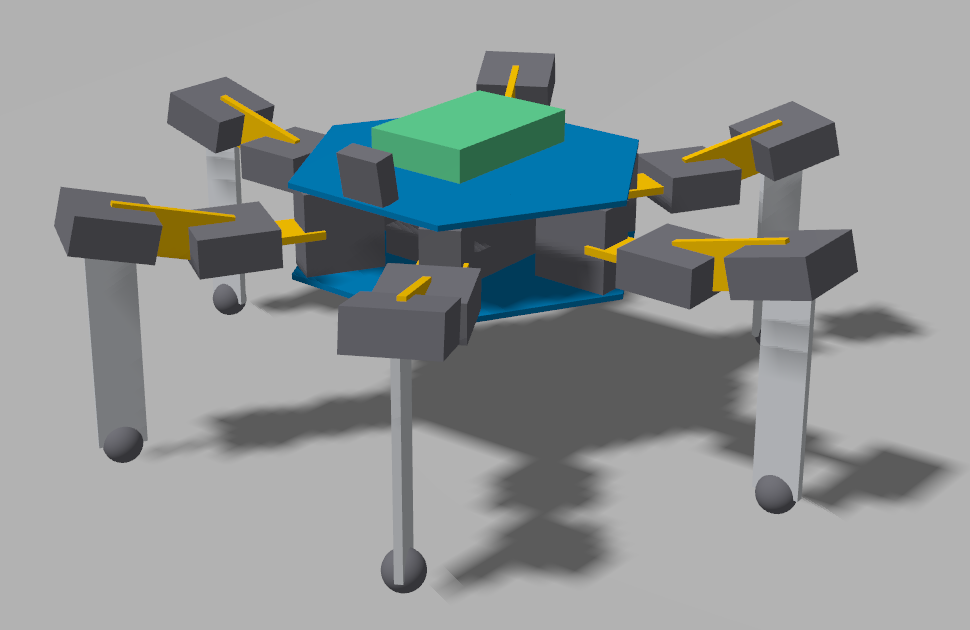
\includegraphics[width=\linewidth]{render_iso_pie.png}\par
\vspace{0.5cm}
\begin{tabularx}{\linewidth}{@{}lY@{}}
\textcolor{Gris}{Autor} & Cesar Olivares Lavalovich\\
\textcolor{Gris}{Asignatura} & Open Robotics — Universidad de Santiago de Chile\\
\textcolor{Gris}{Profesor} & José Pascal\\
\textcolor{Gris}{Fecha} & Noviembre de 2026 · versión 1.0\\
\textcolor{Gris}{Repositorio} & \texttt{Evaluacion1\_version\_Hexapodo/} (rama \texttt{hexapodo})\\
\end{tabularx}
\vfill

\includegraphics[height=1.3cm]{usach_logo.jpg}
\end{titlepage}
\setcounter{page}{2}

%======================================================== ÍNDICE
\renewcommand{\contentsname}{Índice}
\tableofcontents
\newpage

%======================================================== RESUMEN
\seccion{Resumen ejecutivo}

Este informe presenta un hexápodo de 18 articulaciones desarrollado como
versión paralela de la Evaluación~1 de Open Robotics. Cumple la misma pauta
que la entrega oficial (el brazo Octavius), pero con un robot con patas, y
suma un aporte propio: \textbf{calcular las dimensiones ideales del robot
real} a partir de los componentes que ya existen (18 servos MG996R, una
Raspberry Pi~4, dos PCA9685 y una LiPo 3S). Todo el trabajo es en
simulación.

\begin{destacado}[title=Resultados principales]
\begin{itemize}[leftmargin=12pt]
  \item \textbf{Robot completo en ROS\,2 Jazzy y Gazebo Harmonic}: modelo
  URDF/xacro de 1,876~kg con las masas reales, 18 articulaciones controladas
  con \texttt{ros2\_control}, IMU y cámara frontal.
  \item \textbf{Se para solo y camina}: marcha trípode con cinemática inversa
  en las 6 patas; avanza, retrocede, va de lado y gira, a 85--91\,\% de la
  velocidad pedida (criterio: más de 80\,\%).
  \item \textbf{Teclado y joystick micro-ROS}: el joystick (ESP32 o ESP32-S3)
  da control proporcional y suave. Todo el lado ROS está probado; falta solo
  la prueba con la placa física, que aún no se compra.
  \item \textbf{Cotas para fabricar}: coxa 45~mm, fémur 60~mm, tibia 115~mm
  (de eje a eje) y radio del cuerpo 80~mm. El diseño de partida sobrecargaba
  el servo del fémur; el nuevo tiene factor de seguridad 2,14 y un modelo de
  torque que coincide al milésimo con Gazebo.
  \item \textbf{Reproducible}: un solo comando instala y compila; 80 tests
  automáticos y una prueba de integración de 8 puntos pasan en el PC de
  desarrollo y en un contenedor \texttt{ros:jazzy} vacío.
\end{itemize}
\end{destacado}

\textbf{Estado de la pauta}: 13 de 14 requisitos cumplidos y verificados; el
de micro-ROS (R9) está completo del lado del software y espera la placa.
\textbf{Entregables}: 21 de 22 (falta D17, el joystick físico).

\subsec{Cómo leer los datos}

Cada número del informe lleva su origen: \textbf{medido} (pesado o medido por
el autor, o medido en la simulación con un script del repositorio),
\textbf{hoja} (hoja de datos del fabricante), \textbf{hipótesis} (estimación
propia, a revisar en el robot real) o \textbf{estudio} (resultado del estudio
de dimensiones). Los términos técnicos se explican la primera vez y se
reúnen en el glosario al final.

%======================================================== CONTEXTO
\seccion{Contexto y alcance}

\subsec{Motivación}

La pauta de la Evaluación~1 pide un ``robot articulado'' simulado en ROS\,2
con Gazebo, \texttt{ros2\_control}, sensores y micro-ROS. La entrega oficial
es un brazo manipulador. Este proyecto repite la pauta con un hexápodo
porque el autor está construyendo uno real: la simulación sirve para
aprender, para cumplir la pauta y, sobre todo, para \textbf{decidir las
medidas de las piezas antes de fabricarlas}. Las piezas que se habían
diseñado ``a ojo'' se descartaron; solo se conservan los adaptadores
coaxiales de los servos.

\subsec{Alcance}

\begin{tabularx}{\linewidth}{@{}lY@{}}
\toprule
\textbf{Incluye} & Modelo, simulación, control, marcha, sensores, teleoperación por teclado y joystick (software y firmware), estudio de dimensiones, pruebas y documentación.\\
\textbf{No incluye} & Construir el robot real, la electrónica de potencia ni el driver de las PCA9685. Quedan como recomendaciones en «Supuestos y trabajo futuro».\\
\bottomrule
\end{tabularx}

\subsec{Componentes reales}

\begin{table}[H]\centering\small
\caption{Componentes del robot real usados en el modelo.}\label{tab:componentes}
\begin{tabularx}{\linewidth}{@{}lYl@{}}
\toprule
\textbf{Componente} & \textbf{Dato usado} & \textbf{Origen}\\\midrule
18 × servo MG996R con eje coaxial & 55~g con adaptadores; 40,7 × 19,7 × 42,9~mm & medido / hoja\\
 & bloqueo 11~kgf·cm = 1,08~N·m a 6~V (9,4~kgf·cm a 4,8~V); 0,14~s/60° & hoja \cite{mg996r}\\
LiPo 3S 5200~mAh 60C & 271~g; 137 × 43 × 22~mm & medido\\
Raspberry Pi~4 & 86~g; 85 × 56~mm & medido / hoja\\
2 × PCA9685 (16 canales) & 9~g c/u; 62 × 25~mm & medido / hoja\\
IMU BNO085 (por comprar) & orientación fusionada en el chip; 3~g & hoja \cite{bno085} / hipótesis\\
Pi Camera Module 3 (por comprar) & campo de visión horizontal 66°; 4~g & hoja \cite{picam3} / hipótesis\\
Estructura, cables, reguladores & 400~g + 100~g & hipótesis\\
\bottomrule
\end{tabularx}
\end{table}

\subsec{Requisitos de la pauta}

\begin{table}[H]\centering\small
\caption{Trazabilidad de la pauta: cómo se cumple y cómo se comprueba cada requisito.}\label{tab:pauta}
\begin{tabularx}{\linewidth}{@{}lYYc@{}}
\toprule
\textbf{\#} & \textbf{Requisito} & \textbf{Cómo se cumple} & \textbf{Estado}\\\midrule
R1 & Paquete con sus directorios & 3 paquetes: \texttt{hexapod\_description}, \texttt{\_control}, \texttt{\_bringup} & \ok\\
R2 & Robot articulado en URDF/xacro & Cuerpo hexagonal + macro de pata ×6 = 18 articulaciones & \ok\\
R3 & Modelo en RViz & \texttt{display.launch.py} & \ok\\
R4 & \texttt{joint\_state\_publisher} & 18 sliders & \ok\\
R5 & Percepción en RViz (modelo, TF) & RobotModel, TF e imagen de la cámara & \ok\\
R6 & Modelo en Gazebo & Base flotante; de pie 60~s a altura estable & \ok\\
R7 & Al menos 2 sensores & IMU (100~Hz) y cámara (15~Hz) & \ok\\
R8 & \texttt{ros2\_control} + teclado & Teclado → marcha → IK → 18 ángulos & \ok\\
R9 & Control con micro-ROS & ESP32 + joystick → \texttt{/hexapod/joystick}; probado con el tópico simulado & \textcolor{Orange}{\bfseries placa}\\
R10 & Todo con un launch & \texttt{bringup.launch.py} & \ok\\
R11 & Estructura de carpetas & Estándar ROS\,2 & \ok\\
R12 & Presentación & Pendiente (E9) & \textcolor{Orange}{\bfseries E9}\\
R13 & Tutorial & Este informe + guía desde cero + inicio rápido & \ok\\
R14 & Entrega reproducible & \texttt{instalar.sh}; prueba en un PC limpio & \ok\\
\bottomrule
\end{tabularx}
\end{table}

\subsec{Etapas del trabajo}

El trabajo se ordenó en etapas, cada una con entregables comprobables. El
color de cada etiqueta indica el tipo de trabajo y se mantiene en todo el
informe.

\begin{table}[H]\centering\small
\caption{Etapas y entregables (D1--D22). Un entregable cuenta solo si su evidencia existe.}\label{tab:etapas}
\begin{tabularx}{\linewidth}{@{}lYl@{}}
\toprule
\textbf{Etapa} & \textbf{Contenido} & \textbf{Entregables}\\\midrule
\etapa{E0} \etapa{E1} & Workspace, parámetros; una pata y su cinemática & D1--D4 \ok\\
\etapa{E2} & Hexápodo completo en RViz & D5--D7 \ok\\
\etapa[Verde]{E3} & De pie en Gazebo & D8--D9 \ok\\
\etapa[MediumBlue]{E4} & Marcha trípode y teclado & D10--D11 \ok\\
\etapa[LightBlue]{E5} & Sensores: IMU y cámara & D12--D13 \ok\\
\etapa[Orange]{E6} & micro-ROS: joystick ESP32 & D14--D16 \ok, D17 placa\\
\etapa[Gris]{E7} & Integración y prueba en limpio & D18--D19 \ok\\
\etapa[Rojo]{E8} & Estudio de dimensiones & D20--D22 \ok\\
\etapa[Gris]{E9} \etapa[Gris]{E10} & Entrega; guía de estudio & este informe\\
\bottomrule
\end{tabularx}
\end{table}

%======================================================== ARQUITECTURA
\seccion{Arquitectura del software}

\subsec{Conceptos de ROS\,2}

ROS\,2 divide un robot en programas pequeños, los \textbf{nodos}, que se
comunican por \textbf{tópicos}: canales con nombre por donde viajan
\textbf{mensajes} de un tipo definido \cite{ros2}. Quien publica no sabe
quién escucha. Así, cada pieza se cambia sin tocar las otras: el teclado y
el joystick publican en el mismo tópico de velocidad, y al nodo que mueve
las patas le da lo mismo quién le habla.

\subsec{Los tres paquetes}

\begin{table}[H]\centering\small
\caption{Paquetes del workspace. Cada uno cambia por motivos distintos.}\label{tab:paquetes}
\begin{tabularx}{\linewidth}{@{}>{\ttfamily\small}lYY@{}}
\toprule
\textbf{Paquete} & \textbf{Contenido} & \textbf{Cambia cuando…}\\\midrule
\texttt{hexapod\_description} & El cuerpo: URDF/xacro, parámetros, RViz & cambian las medidas o piezas\\
\texttt{hexapod\_control} & El cerebro: cinemática, marcha, estudio de dimensiones (sin ROS) y los nodos & cambia cómo se mueve\\
\texttt{hexapod\_bringup} & El arranque: Gazebo, controladores, puentes, configuración & cambia cómo se simula o arranca\\
\bottomrule
\end{tabularx}
\end{table}

La lógica (cinemática, marcha, estudio) está en módulos \textbf{sin ROS}:
se prueba en milisegundos sin abrir el simulador. Los nodos solo la conectan
con los tópicos.

\subsec{Nodos y tópicos}

\begin{figure}[H]\centering
\resizebox{\linewidth}{!}{%
\begin{tikzpicture}[font=\footnotesize,
  nodo/.style={draw=DarkBlue,fill=white,rounded corners=3pt,minimum height=9mm,minimum width=2.7cm,align=center,line width=0.9pt},
  ext/.style={nodo,draw=Orange},
  flecha/.style={-{Stealth[length=2.2mm]},line width=0.75pt,color=DarkGray},
  top/.style={font=\scriptsize\ttfamily,color=MediumBlue,inner sep=1.5pt}]
% fila 1: entradas
\node[ext] (esp) at (0,0) {ESP32 + joystick\\\scriptsize micro-ROS, USB};
\node[nodo] (agent) at (4.8,0) {micro\_ros\_agent};
\node[nodo] (j2t) at (10.4,0) {joy\_to\_twist};
\node[nodo] (kb) at (10.4,-1.8) {keyboard\_teleop\\\scriptsize (otra terminal)};
\node[nodo,minimum width=2.4cm] (gait) at (15.0,-0.9) {gait\_node\\\scriptsize marcha + IK};
\draw[flecha] (esp) -- node[top,above]{XRCE-DDS} (agent);
\draw[flecha] (agent) -- node[top,above]{/hexapod/joystick} (j2t);
\draw[flecha] (j2t.east) -- node[top,above,sloped]{/hexapod/cmd\_vel} (gait.north west);
\draw[flecha] (kb.east) -- node[top,below,sloped]{/hexapod/cmd\_vel} (gait.south west);
% Gazebo
\node[nodo,minimum width=3.6cm] (sens) at (3.2,-4.1) {sensores simulados\\\scriptsize cámara · IMU · odometría};
\node[nodo,minimum width=4.3cm] (cm) at (11.6,-4.1) {controller\_manager\\\scriptsize legs\_controller · joint\_state\_broadcaster};
\begin{scope}[on background layer]
\node[draw=Verde,line width=1pt,rounded corners=4pt,fit=(cm)(sens),inner xsep=8pt,inner ysep=11pt] (gzb) {};
\end{scope}
\node[font=\footnotesize\bfseries,color=Verde,anchor=north west] at (gzb.north west) {Gazebo Harmonic};
\draw[flecha] (gait.south) |- node[top,pos=0.3,right,align=left]{/legs\_controller/\\commands\\(18 ángulos, 50 Hz)} (cm.east);
% salidas
\node[nodo] (rsp) at (11.6,-6.5) {robot\_state\_publisher};
\node[nodo] (rviz) at (3.2,-6.5) {RViz};
\draw[flecha] (cm) -- node[top,right]{/joint\_states} (rsp);
\draw[flecha] (rsp) -- node[top,above]{/tf (marcos del robot)} (rviz);
\draw[flecha] (sens) -- node[top,right,align=left,pos=0.62]{ros\_gz\_bridge: /hexapod/imu,\\camera/image, /hexapod/odom,\\/tf (odom → base\_link)} (rviz);
\end{tikzpicture}}
\caption{Nodos (cajas) y tópicos (texto en azul). Naranjo: hardware externo; verde: lo que corre dentro de Gazebo.}\label{fig:nodos}
\end{figure}

\begin{table}[H]\centering\small
\caption{Tópicos principales.}\label{tab:topicos}
\begin{tabularx}{\linewidth}{@{}>{\ttfamily\footnotesize}l>{\ttfamily\footnotesize}lcY@{}}
\toprule
\textbf{Tópico} & \textbf{Mensaje} & \textbf{Hz} & \textbf{Publica → escucha}\\\midrule
\texttt{/hexapod/joystick} & \texttt{sensor\_msgs/Joy} & 20 & ESP32 → \texttt{joy\_to\_twist}\\
\texttt{/hexapod/cmd\_vel} & \texttt{geometry\_msgs/Twist} & 10--20 & joystick o teclado → \texttt{gait\_node}\\
\texttt{/legs\_controller/commands} & \texttt{Float64MultiArray} & 50 & \texttt{gait\_node} → controlador (18 ángulos)\\
\texttt{/joint\_states} & \texttt{sensor\_msgs/JointState} & 100 & controlador → \texttt{robot\_state\_publisher}\\
\texttt{/hexapod/imu} & \texttt{sensor\_msgs/Imu} & 100 & Gazebo → ROS (puente)\\
\texttt{/hexapod/camera/image} & \texttt{sensor\_msgs/Image} & 15 & Gazebo → RViz\\
\texttt{/hexapod/odom} & \texttt{nav\_msgs/Odometry} & 50 & Gazebo → scripts de medición\\
\bottomrule
\end{tabularx}
\end{table}

\textbf{Tiempo simulado.} Todos los nodos usan el reloj de Gazebo
(\texttt{/clock}) y no el del PC. Si el PC es lento, la simulación va más
lenta pero todo sigue sincronizado.

\subsec{Arranque en un comando}

\texttt{bringup.launch.py} levanta todo. Dentro, \texttt{gazebo.launch.py}
usa eventos para respetar el orden: el robot tiene que existir antes de
activar \path{joint_state_broadcaster}; este, antes que
\path{legs_controller}; y este, antes que \texttt{gait\_node}. Con
\texttt{use\_microros:=true} se lanza también el agente micro-ROS.

%======================================================== MODELO
\seccion{Modelo del robot}

\subsec{URDF y xacro}

El \textbf{URDF} describe el robot como un árbol de \textbf{links} (piezas
rígidas con forma, colisión, masa e inercia) unidos por \textbf{joints}
(articulaciones). \textbf{xacro} agrega variables, cuentas y macros: la pata
se escribe una vez y se usa seis veces. Sin xacro el modelo serían unas
1500 líneas de XML repetido.

\begin{table}[H]\centering\small
\caption{Archivos del modelo.}\label{tab:xacro}
\begin{tabularx}{\linewidth}{@{}>{\raggedright\arraybackslash\ttfamily\small}p{5.2cm}Y@{}}
\toprule
\textbf{Archivo} & \textbf{Rol}\\\midrule
\texttt{hexapod.urdf.xacro} & Arma el robot: incluye todo e instancia las 6 patas\\
\texttt{hexapod\_params.xacro} & \textbf{Única fuente de verdad}: todas las medidas y masas, con su origen\\
\texttt{leg.xacro} & Macro de una pata: coxa, fémur, tibia y pie\\
\texttt{body.xacro} & Cuerpo hexagonal y servos de las coxas\\
components.xacro\newline sensors.xacro & Batería, Raspberry, PCA9685; IMU y cámara\\
ros2\_control.xacro\newline gazebo.xacro\newline sensors\_gazebo.xacro & Interfaces de control, contacto de los pies y plugins de los sensores\\
\bottomrule
\end{tabularx}
\end{table}

\subsec{Cuerpo y patas}

El cuerpo es un \textbf{hexágono regular horizontal} formado por dos placas
separadas 45~mm (justo el alto del servo). Las patas salen de los vértices,
a $\pm 30^\circ$, $\pm 90^\circ$ y $\pm 150^\circ$; el frente mira a un lado
plano. URDF no tiene hexágonos, así que cada placa se arma con tres
rectángulos girados $0^\circ$, $60^\circ$ y $120^\circ$, cuyas esquinas son
los vértices.

Cada pata tiene tres articulaciones: la \textbf{coxa} gira en torno al eje
vertical (adelante/atrás), el \textbf{fémur} sube y baja la pata, y la
\textbf{tibia} dobla la rodilla. La articulación de cada coxa se gira el
ángulo de su vértice, de modo que en el marco de cada pata el eje $x$ apunta
siempre hacia afuera: \textbf{la misma cinemática sirve para las seis}.

\begin{figure}[H]\centering
\begin{minipage}{0.49\linewidth}\centering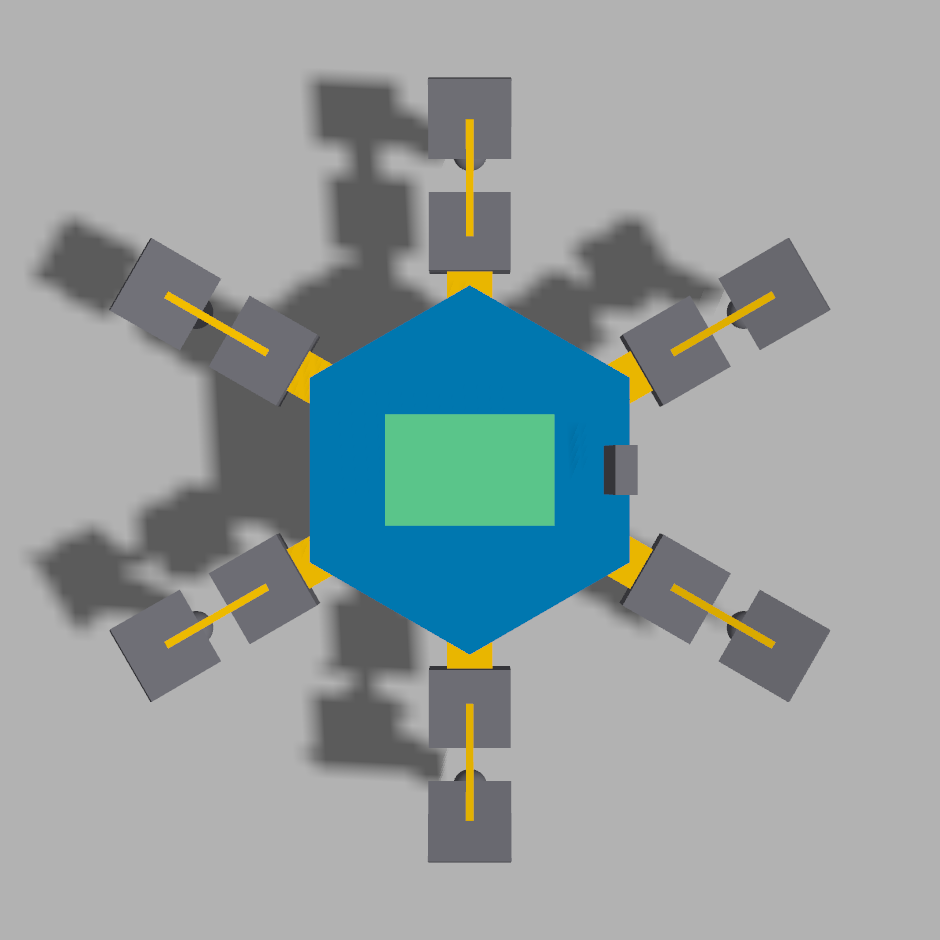
\includegraphics[width=\linewidth]{render_top_pie.png}\end{minipage}\hfill
\begin{minipage}{0.49\linewidth}\centering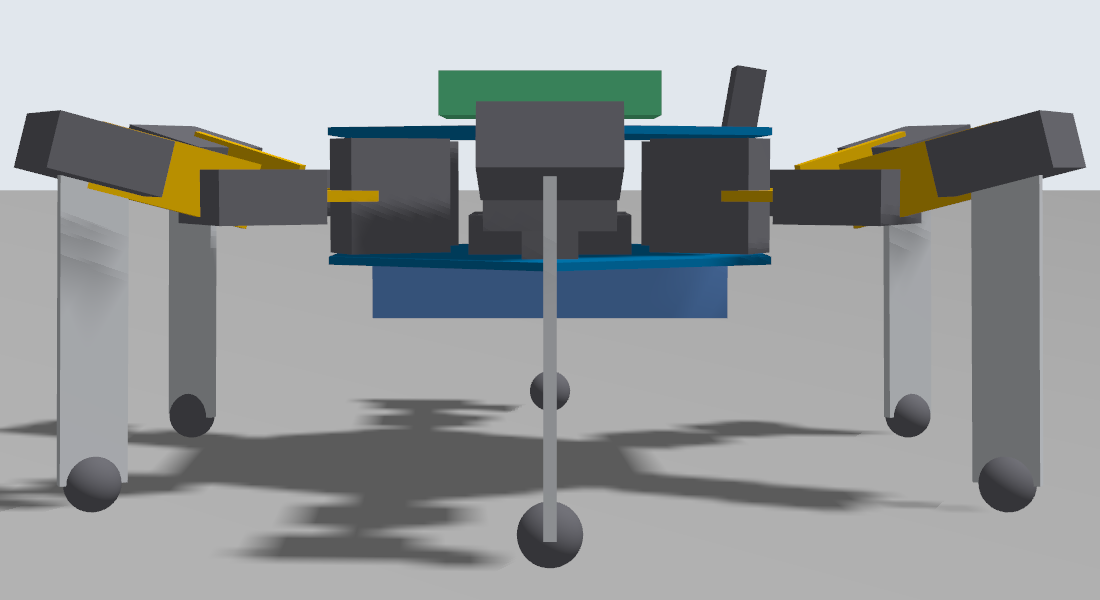
\includegraphics[width=\linewidth]{render_side_pie.png}\end{minipage}
\caption{El modelo en Gazebo, de pie. Izquierda: vista superior (frente a la derecha; la caja verde es la Raspberry Pi y la pequeña al frente, la cámara). Derecha: vista lateral; la batería (azul) cuelga bajo el cuerpo.}\label{fig:renders}
\end{figure}

\subsec{Layout y masa}

\begin{table}[H]\centering\small
\caption{Ubicación de los componentes y por qué.}\label{tab:layout}
\begin{tabularx}{\linewidth}{@{}lY@{}}
\toprule
\textbf{Componente} & \textbf{Dónde y por qué}\\\midrule
Batería & Bajo la placa inferior: es la masa mayor después de los servos y abajo baja el centro de masa. Entre las placas no cabe\\
Raspberry Pi~4 & Sobre la placa superior: acceso a puertos y a la cámara. En el robot real es el controlador\\
PCA9685 ×2 & Entre las placas, al centro: izquierda (0x40) y derecha (0x41)\\
IMU & En el centro del cuerpo: mide la orientación sin aceleraciones extra por giro\\
Cámara & Lado frontal, 10° hacia el suelo: ve el terreno que viene\\
\bottomrule
\end{tabularx}
\end{table}

La masa del modelo es \textbf{1,876~kg} y el centro de masa queda a menos de
5~mm del eje vertical (ambos comprobados por test). El árbol de marcos (TF)
cuelga de \texttt{base\_link}, el centro del cuerpo, con la convención
REP-103: $x$ adelante, $y$ izquierda, $z$ arriba, en metros y radianes
\cite{rep103}.

\begin{figure}[btp]\centering
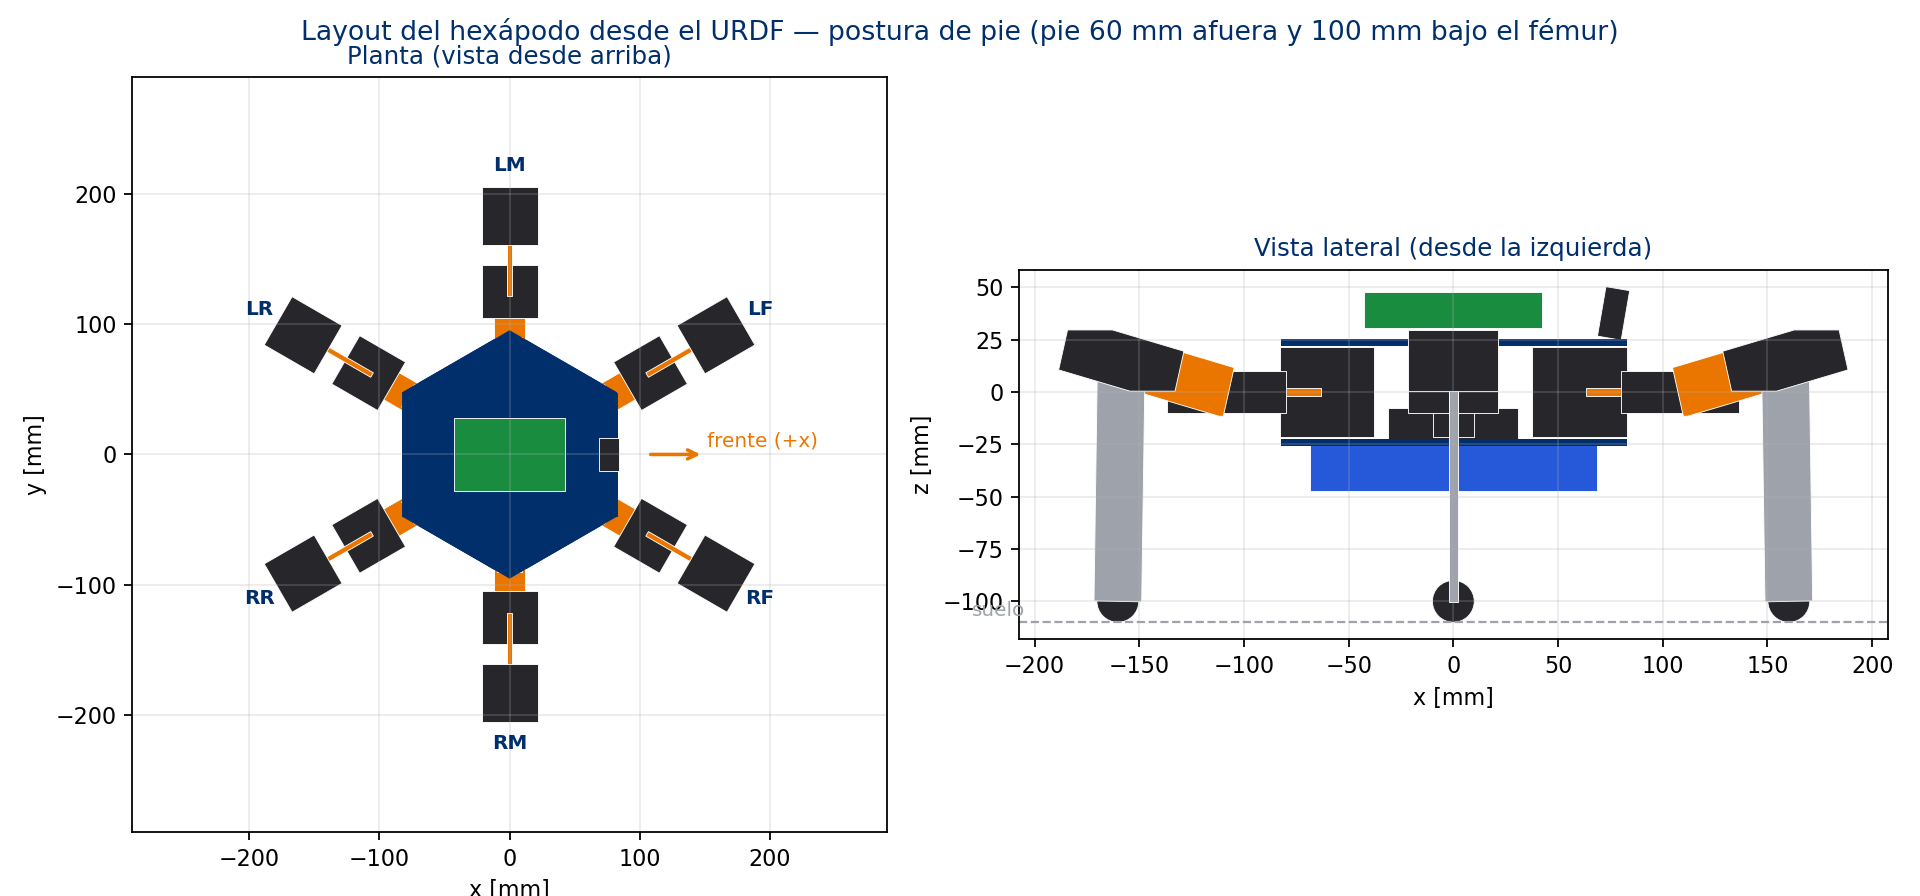
\includegraphics[width=0.9\linewidth]{layout.png}
\caption{Layout generado directamente desde el URDF (\texttt{analysis/plot\_layout.py}): si cambia una medida, la figura cambia.}\label{fig:layout}
\end{figure}

%======================================================== CINEMÁTICA
\seccion{Cinemática de una pata}

En el marco de la pata (origen en el eje de la coxa), con $\theta_1$ coxa,
$\theta_2$ fémur y $\theta_3$ tibia, y largos $L_1, L_2, L_3$:

\textbf{Cinemática directa} (ángulos → posición del pie):
\begin{align}
r &= L_1 + L_2\cos\theta_2 + L_3\cos(\theta_2+\theta_3)\\
x &= r\cos\theta_1,\qquad y = r\sin\theta_1,\qquad z = L_2\sin\theta_2 + L_3\sin(\theta_2+\theta_3)
\end{align}

\textbf{Cinemática inversa} (posición → ángulos), con la rodilla hacia arriba,
por ley de cosenos:
\begin{align}
\theta_1 &= \operatorname{atan2}(y, x),\qquad \rho = \sqrt{x^2+y^2}-L_1,\qquad D^2=\rho^2+z^2\\
\cos\theta_3 &= \frac{D^2 - L_2^2 - L_3^2}{2L_2L_3},\qquad \theta_3 = -\arccos(\cos\theta_3)\\
\theta_2 &= \operatorname{atan2}(z,\rho) - \operatorname{atan2}\!\left(L_3\sin\theta_3,\; L_2 + L_3\cos\theta_3\right)
\end{align}

Si el punto no se alcanza o un ángulo sale de su límite, la función lanza un
error en vez de entregar un ángulo imposible. Los largos y límites se leen
del propio URDF, así que el modelo y la cinemática nunca se contradicen.

\begin{table}[H]\centering\small
\caption{Validación de la cinemática.}\label{tab:cinematica}
\begin{tabularx}{\linewidth}{@{}YYl@{}}
\toprule
\textbf{Prueba} & \textbf{Criterio} & \textbf{Resultado}\\\midrule
Ida y vuelta FK(IK($p$)) en 5000 puntos al azar & error < 0,1~mm & \ok\\
Pie del URDF (transformadas encadenadas) vs.\ FK, 500 poses & error < 0,1~mm & \ok\\
\texttt{tf2\_echo} con todo en 0 & $L_1+L_2+L_3$ & \ok\\
\bottomrule
\end{tabularx}
\end{table}

%======================================================== GAZEBO
\seccion{Simulación: de pie en Gazebo}

\subsec{Base flotante y ros2\_control}

A diferencia de un brazo atornillado a la mesa, nada une el cuerpo al
mundo: el robot se sostiene solo si los pies tocan el suelo, la fricción
impide que resbalen y los servos aguantan el peso. Los pies son esferas con
fricción $\mu = 1$ y un contacto algo blando para que no rebote.

\texttt{ros2\_control} \cite{ros2control} separa el \textbf{hardware} (qué
articulaciones existen y qué interfaces ofrecen: comando de posición;
estado de posición, velocidad y torque) de los \textbf{controladores}. En
simulación el hardware es el plugin \texttt{gz\_ros2\_control}
\cite{gzros2control}, que limita cada articulación al torque (1,08~N·m) y la
velocidad (7,48~rad/s) del MG996R. En el robot real se cambiaría por un
driver de las PCA9685 y todo lo demás quedaría igual.

\subsec{Postura suave}

El robot aparece apoyado en la batería y \texttt{gait\_node} lo levanta en
tres fases: \textbf{recoger} las patas (1~s), \textbf{bajar los pies} en
línea recta con cinemática inversa en cada paso (2,5~s) y \textbf{mantener}
la postura. Las transiciones usan $s(t) = (1-\cos\pi t)/2$, que parte y llega
con velocidad cero.

\begin{figure}[H]\centering
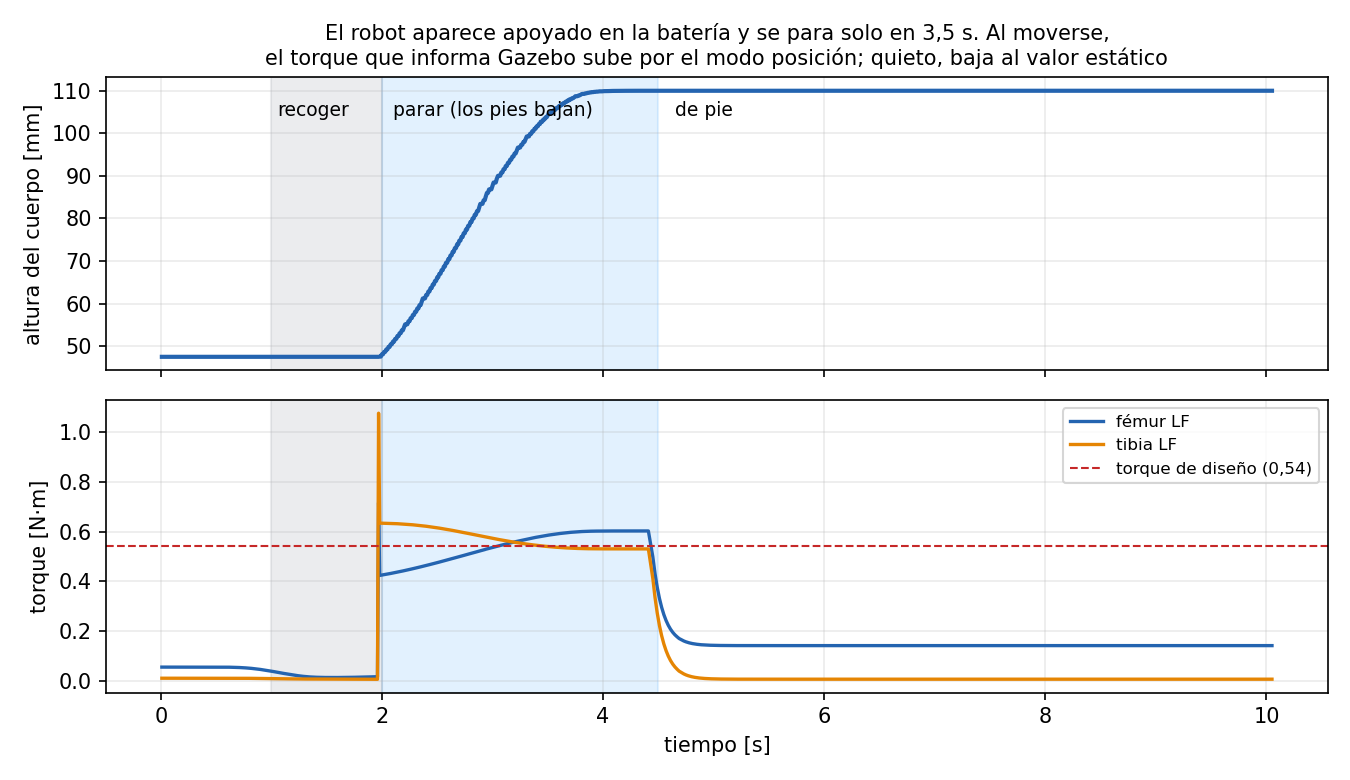
\includegraphics[width=\linewidth]{subida.png}
\caption{Subida medida en Gazebo (\texttt{scripts/registrar\_subida.py}). El cuerpo pasa de 47,5 a 110~mm. Quieto en 6 patas, el fémur hace 0,14~N·m, igual al cálculo.}\label{fig:subida}
\end{figure}

\subsec{Problemas y soluciones}

\begin{table}[H]\centering\small
\caption{Problemas encontrados al ponerlo de pie.}\label{tab:problemas_e3}
\begin{tabularx}{\linewidth}{@{}YY@{}}
\toprule
\textbf{Problema} & \textbf{Solución}\\\midrule
El nodo se detuvo: la postura recogida exigía doblar la rodilla a $-148^\circ$, fuera del límite de $-143^\circ$ & Pie recogido más afuera. La cinemática inversa avisó con un error en vez de mandar un ángulo imposible\\
El robot no se levantaba: el nodo leyó el tiempo antes de que llegara el reloj de Gazebo y pidió la postura de golpe desde las patas estiradas; los pies apoyaron lejos y se trabaron & Esperar el reloj. Lección para el robot real: \textbf{nunca pasar directo de patas estiradas a la postura de pie}\\
\bottomrule
\end{tabularx}
\end{table}

\textbf{Evidencia D8}: 60~s de pie a 110,00~mm, variación ±0,00~mm,
inclinación 0° y deriva 0~mm (\texttt{scripts/medir\_postura.py}).
\textbf{D9}: ambos controladores \emph{active}.

%======================================================== MARCHA
\seccion{Marcha trípode}

\subsec{Cómo funciona}

Las patas forman dos grupos que se alternan: \textbf{A} = LF, RM, LR y
\textbf{B} = RF, LM, RR. Siempre hay un triángulo de tres patas en el suelo,
la forma más rápida de caminar estáticamente estable con seis patas
\cite{wilson1966}. Cada pata tiene una fase $\phi\in[0,1)$ que avanza con el
tiempo, con periodo $T$ y fracción de apoyo $\beta$:

\begin{align}
\text{apoyo }(\phi<\beta):&\quad \mathbf p = \mathbf p_0 + \left(\tfrac12 - \tfrac{\phi}{\beta}\right)\boldsymbol\Delta\\
\text{vuelo }(\phi\ge\beta):&\quad u = \tfrac{\phi-\beta}{1-\beta},\quad \mathbf p = \mathbf p_0 + \left(u-\tfrac12\right)\boldsymbol\Delta + h\sin(\pi u)\,\hat z\\
\text{vector de paso:}&\quad \boldsymbol\Delta = \beta T\left(\mathbf v + \omega\,\hat z\times\mathbf p_0\right)
\end{align}

En el apoyo el pie retrocede respecto del cuerpo, y eso empuja al robot; en
el vuelo vuelve adelante por un arco de altura $h$. El vector de paso
incluye el giro: cada pata da un paso distinto según su posición
$\mathbf p_0$. Cada posición de pie pasa por la cinemática inversa de su
pata y \texttt{gait\_node} publica los 18 ángulos a 50~Hz.

\begin{figure}[H]\centering
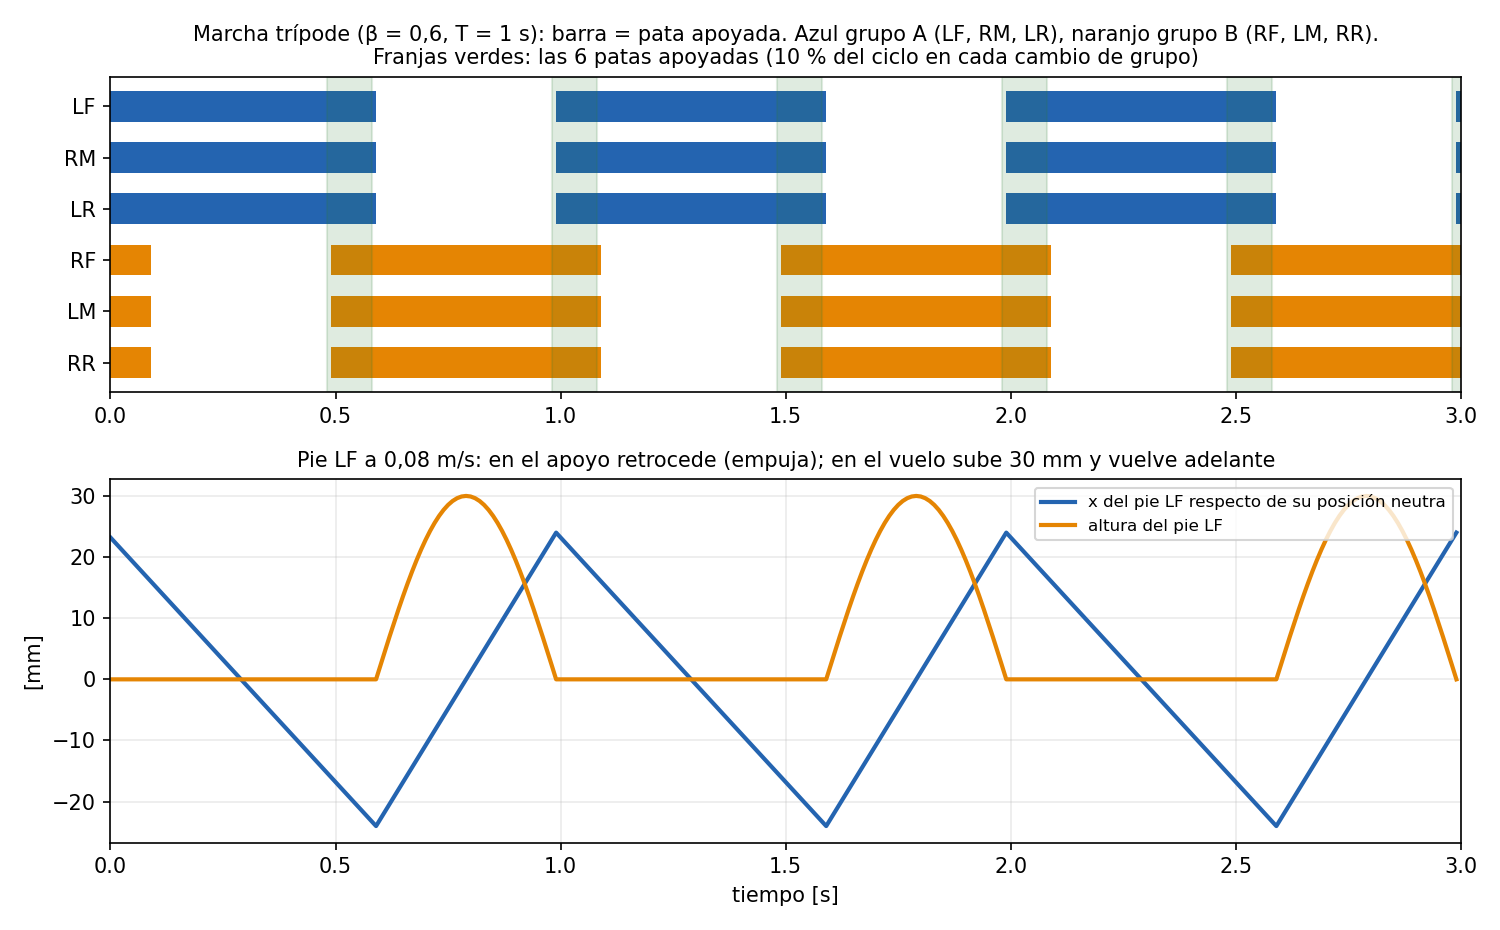
\includegraphics[width=\linewidth]{marcha_tripode.png}
\caption{Arriba: cuándo apoya cada pata. Abajo: trayectoria del pie LF. Calculado con \texttt{gait.py} (\texttt{analysis/figuras\_informe.py}).}\label{fig:marcha}
\end{figure}

\subsec{Decisiones de diseño}

\begin{itemize}
  \item \textbf{Cálculo incremental.} Las fórmulas cerradas hacen saltar el
  pie si la velocidad cambia a mitad de paso. Se calcula paso a paso: el pie
  apoyado sigue desde donde está. Con velocidad constante el resultado es
  idéntico a las fórmulas (un test lo comprueba).
  \item \textbf{Rampa}: la velocidad cambia como máximo 0,4~m/s².
  \item \textbf{Velocidad máxima de 0,10~m/s}: no se eligió por estabilidad,
  es el tope geométrico. Un pie recorre $\beta T v$ por paso y no puede pasar
  de 60~mm sin salir del alcance: $v_{\max} = 0{,}06/(0{,}6\times1) = 0{,}10$~m/s.
  \item \textbf{$\beta = 0{,}6$ en vez de 0,5.} Ver tabla~\ref{tab:beta}.
\end{itemize}

\begin{table}[H]\centering\small
\caption{Ajustes de la marcha en Gazebo.}\label{tab:beta}
\begin{tabularx}{\linewidth}{@{}lYY@{}}
\toprule
\textbf{Prueba} & \textbf{Resultado} & \textbf{Decisión}\\\midrule
$\beta = 0{,}5$ (trípode puro) & 22--26\,\% más lento de lo pedido; el cuerpo cae 5~mm en cada cambio de grupo & Un grupo despega en el mismo instante en que el otro aterriza, y los servos se atrasan\\
Ganancia del servo simulado 0,5 & De pie bien; caminando se desploma & Se mantiene la de fábrica (0,1)\\
$\beta = 0{,}6$ & Las 6 patas apoyan un 10\,\% del ciclo en cada cambio: cae 3~mm; error 9--15\,\% & \textbf{Se adopta} (sigue siendo trípode)\\
\bottomrule
\end{tabularx}
\end{table}

\subsec{Resultados}

\begin{figure}[H]\centering
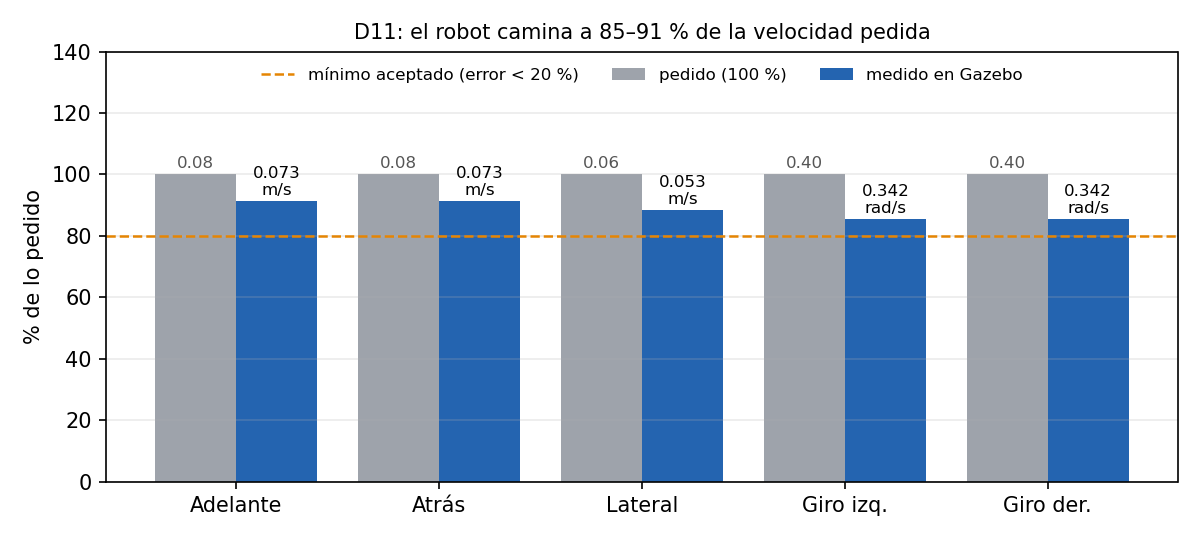
\includegraphics[width=0.92\linewidth]{velocidad_d11.png}
\caption{Velocidad real (odometría de referencia de Gazebo, 10~s por prueba) frente a la pedida (\texttt{scripts/medir\_marcha.py}).}\label{fig:d11}
\end{figure}

\begin{destacado}[title=El torque caminando no es la carga real]
Caminando, Gazebo informa ~1,07~N·m en el fémur durante todo el apoyo, con
un error de posición de solo 0,02~rad. No es el peso: en modo posición,
\texttt{gz\_ros2\_control} \textbf{impone una velocidad} a cada articulación
usando hasta todo el torque disponible, y las tres patas apoyadas, con los
pies fijos por la fricción, se empujan entre sí. La figura~\ref{fig:subida}
muestra el mismo efecto al subir. Por eso los torques de diseño se calculan
con un modelo estático, que sí se validó (ver «Estudio de dimensiones»).
\end{destacado}

\begin{figure}[H]\centering
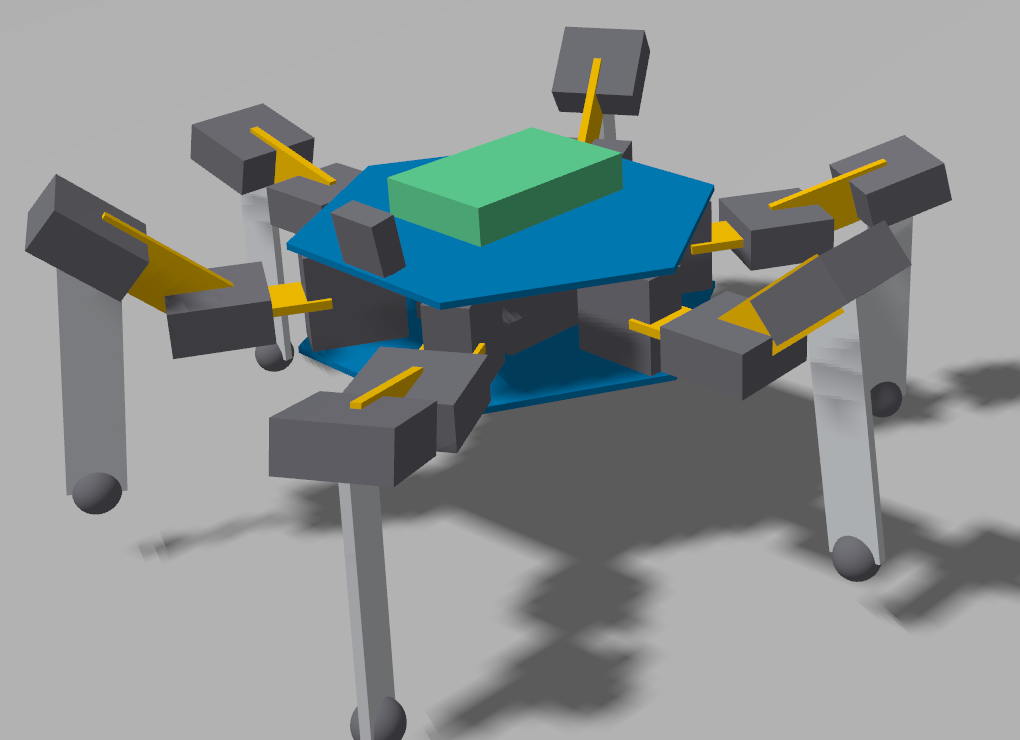
\includegraphics[width=0.85\linewidth]{render_iso_marcha.png}
\caption{Caminando hacia adelante: el grupo B en el aire y el grupo A apoyado.}\label{fig:render_marcha}
\end{figure}

%======================================================== SENSORES
\seccion{Sensores}

Cada sensor tiene dos partes: un link que lo ubica en el robot y un bloque
de Gazebo que dice qué mide y en qué tópico. \texttt{ros\_gz\_bridge}
\cite{rosgz} pasa los datos a ROS\,2.

\begin{itemize}
  \item \textbf{IMU} (BNO085): orientación, velocidad angular y aceleración a
  100~Hz, con ruido gaussiano del orden de la hoja (giroscopio
  0,005~rad/s, acelerómetro 0,03~m/s²; \emph{hipótesis}).
  \item \textbf{Cámara} (Pi Camera Module 3): modelo estenopeico, 640 × 480 a
  15~Hz. Con campo de visión horizontal de 66° \cite{picam3}, la focal en
  píxeles es $f_x = (W/2)/\tan(\mathrm{HFOV}/2) = 320/\tan 33^\circ \approx 493$~px.
  La imagen sale en el marco óptico ($z$ adelante, $x$ derecha, $y$ abajo).
\end{itemize}

\begin{minipage}[c]{0.53\linewidth}\small
\begin{tabular}{@{}l@{\hspace{6pt}}r@{}}
\toprule
\textbf{Comprobación} & \textbf{Resultado}\\\midrule
IMU & 100,0~Hz \ok\\
Gravedad (quieta) & 9,811~m/s² \ok\\
Ruido giroscopio & 0,0050~rad/s \ok\\
Giro 5~s: IMU / odom. & 97,6° / 98,0° \ok\\
Cámara & 14,9~Hz, 640 × 480 \ok\\
Focal (\texttt{camera\_info}) & 492,8~px \ok\\
\bottomrule
\end{tabular}
\end{minipage}\hfill
\begin{minipage}[c]{0.43\linewidth}
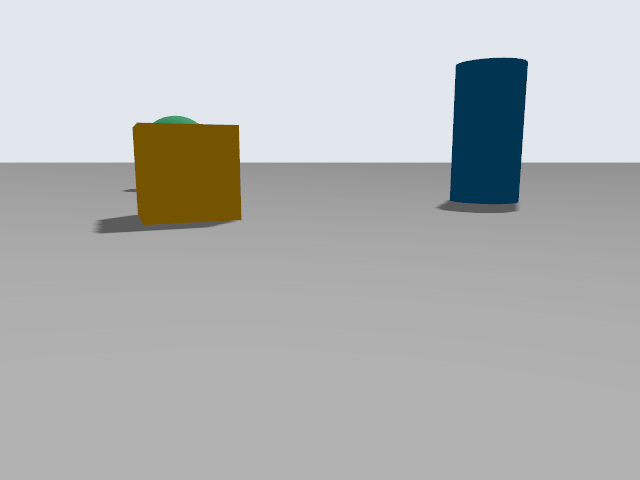
\includegraphics[width=\linewidth]{camara_frontal.png}
\captionof{figure}{Imagen de la cámara frontal: la caja a la izquierda del robot sale a la izquierda.}\label{fig:camara}
\end{minipage}

%======================================================== MICRO-ROS
\seccion{Teleoperación y micro-ROS}

\subsec{Cadena del joystick}

micro-ROS \cite{microros} lleva ROS\,2 a microcontroladores. La ESP32 no
puede correr DDS, el sistema de comunicación de ROS\,2: habla un protocolo
liviano por USB con el \textbf{agente} del PC, que la presenta al resto
como un nodo más. La placa solo lee los dos ejes y el botón, los normaliza a
$[-1,1]$ y publica \texttt{sensor\_msgs/Joy} a 20~Hz. \textbf{Las decisiones
están en ROS}, donde se ajustan sin reprogramar la placa.

\subsec{Control proporcional y suave}

La palanca entrega valores continuos. \texttt{joy\_to\_twist} los convierte
en velocidad en tres pasos:
\begin{align}
\text{zona muerta: } x' &= \operatorname{signo}(x)\,\frac{|x|-d}{1-d}\quad (|x|>d),\qquad d = 0{,}08\\
\text{curva expo: } y &= (1-e)\,x' + e\,x'^3,\qquad e = 0{,}5\\
\text{escala: } v &= y\,v_{\max}
\end{align}
Bajo el 8\,\% de la palanca no pasa nada (un potenciómetro suelto nunca marca
0 exacto). Sobre ese umbral la salida parte de 0 sin salto. La curva expo da
control fino cerca del centro y llega a la velocidad máxima en el tope, y la
rampa de la marcha suaviza los cambios bruscos. El botón cambia el eje
horizontal entre \textbf{girar} y \textbf{caminar de lado}. Si la placa se
desconecta, el robot se detiene solo en 0,5~s.

\begin{figure}[H]\centering
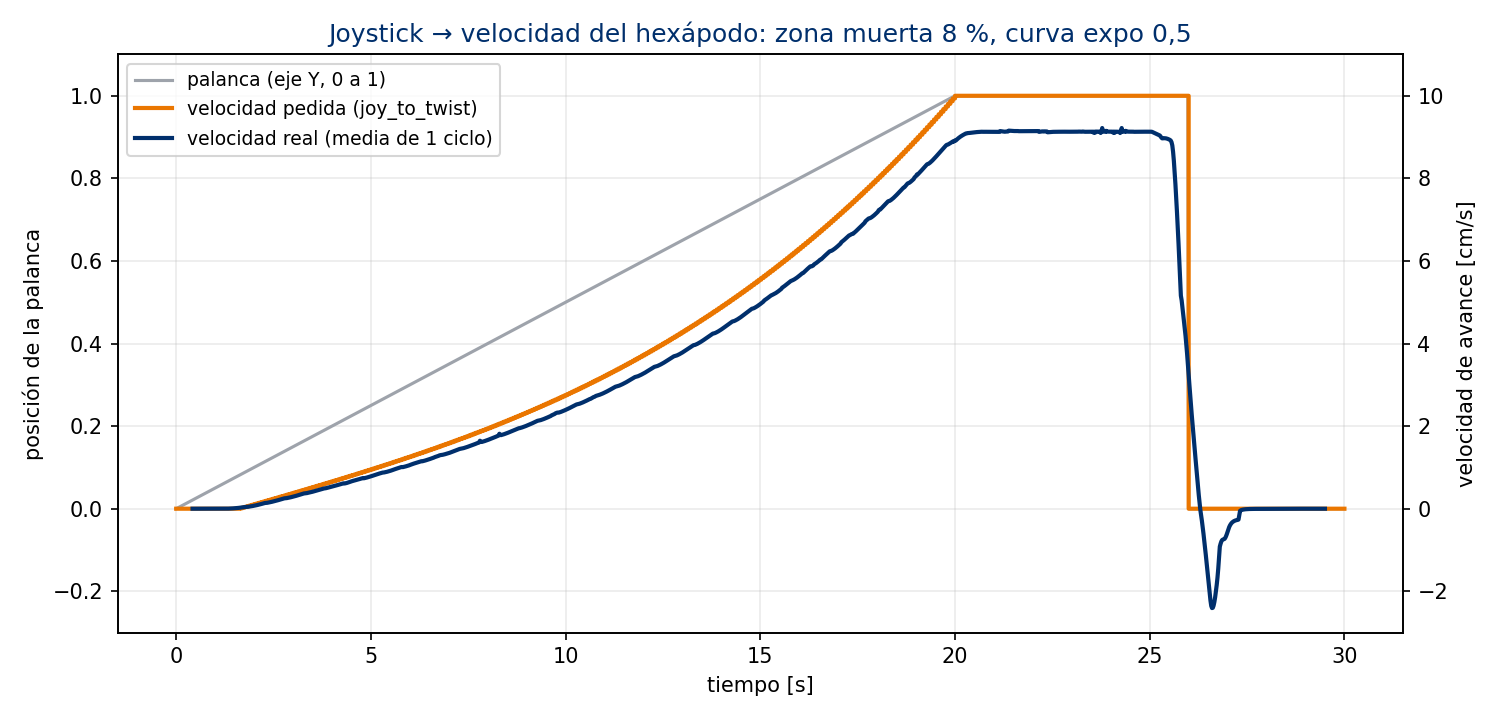
\includegraphics[width=\linewidth]{joystick_gradiente.png}
\caption{Palanca movida de a poco de 0 al tope (joystick simulado a 20~Hz, igual que la ESP32). La velocidad real sigue a la pedida; al tope logra 9,1 de 10~cm/s.}\label{fig:joystick}
\end{figure}

\subsec{Firmware}

Un mismo archivo sirve para ESP32 y ESP32-S3; los pines se eligen según la
placa al compilar. Para la ESP32 clásica compila con el Arduino IDE y la
librería \texttt{micro\_ros\_arduino}, sin errores ni advertencias (30\,\% de
la memoria de programa). Esa librería solo trae micro-ROS precompilado para
la ESP32 clásica, así que para la S3 se usa PlatformIO con
\path{micro_ros_platformio} \cite{microrospio}, que compila micro-ROS
para la placa (12,8\,\% de RAM). La conexión, la carga y una lista de 12
pasos para la prueba con hardware están en
\path{docs/joystick_esp32.md}.

%======================================================== ESTUDIO
\seccion{Estudio de dimensiones}

\subsec{Pregunta y requisitos}

\begin{destacado}[title=Pregunta]
Con 18 MG996R, la LiPo y la electrónica dadas, ¿qué largos de coxa, fémur
y tibia, y qué radio del cuerpo, permiten caminar con margen de torque, sin
choques, con altura libre y de forma estable?
\end{destacado}

\begin{table}[H]\centering\small
\caption{Requisitos del estudio.}\label{tab:requisitos}
\begin{tabularx}{\linewidth}{@{}>{\raggedright\arraybackslash}p{4.4cm}>{\raggedright\arraybackslash}p{3.4cm}Y@{}}
\toprule
\textbf{Requisito} & \textbf{Valor} & \textbf{Por qué}\\\midrule
Paso & 60~mm & 0,10~m/s con la marcha actual\\
Altura de vuelo & 30~mm & pasar obstáculos chicos\\
Altura libre bajo la batería & $\ge$ 60~mm & propuesta del plan\\
Factor de seguridad del torque & $\ge$ 2 & los MG996R reales, sobre todo las copias, rinden menos que la hoja\\
Margen de estabilidad & $\ge$ 40~mm & centro de masa lejos del borde del trípode\\
Sin choques & pies $\ge$ 30~mm; servos $\ge$ 5~mm & entre patas vecinas\\
Pata sin estirar del todo & $D \le 0{,}9\,(L_2+L_3)$ & lejos de la pata recta\\
Distancia a los topes & $\ge$ 0,1~rad & no trabajar contra el tope\\
Rodilla sobre el fémur en el apoyo & $\ge$ 0 & el servo de la rodilla no roza el suelo\\
\bottomrule
\end{tabularx}
\end{table}

\subsec{Modelo de carga}

En la marcha trípode tres patas sostienen todo el peso:
$F = Mg/3 = 1{,}876\times9{,}81/3 = 6{,}13$~N por pie. El torque del fémur es
$F$ por la distancia horizontal del eje del fémur al pie, menos el peso
propio de la pata; el de la tibia, $F$ por la distancia horizontal de la
rodilla al pie. El peor punto es el pie en el extremo exterior del paso:
$d + S/2$. El torque de diseño es la mitad del de bloqueo:
$\tau_d = 1{,}08/2 = 0{,}54$~N·m.

\begin{table}[H]\centering\small
\caption{Validación del modelo contra Gazebo, con el robot quieto en 3 patas (\texttt{scripts/medir\_torque\_tripode.py}).}\label{tab:validacion}
\begin{tabularx}{\linewidth}{@{}Ycc@{}}
\toprule
\textbf{Caso} & \textbf{Modelo fémur / tibia} & \textbf{Gazebo fémur / tibia}\\\midrule
Diseño de partida, pie a 70~mm & 0,374 / 0,025 & 0,375 / 0,025\\
Diseño nuevo, pie a 60~mm (neutro) & 0,325 / 0,012 & 0,325 / 0,012\\
Diseño nuevo, pie a 90~mm (peor punto) & 0,506 / 0,187 & 0,506 / 0,188\\
\bottomrule
\end{tabularx}
\end{table}

\subsec{Método}

\begin{enumerate}
  \item \textbf{Empaque → $L_1$ y $R$.} El servo del fémur no debe tocar la
  placa: $L_1 \ge 15 + 20{,}35 + 5 = 40{,}3$~mm, y se elige \textbf{45~mm}
  (4~mm más para el rodamiento del adaptador coaxial). La batería debe caber
  bajo el hexágono y las PCA9685 no deben tocar los servos de coxa:
  $R \ge 79$~mm, y se elige \textbf{80~mm}.
  \item \textbf{Altura → $H$.} Batería a $\ge$ 60~mm del suelo: $H = 100$~mm.
  \item \textbf{Torque contra estabilidad → $d$.} Abrir la pata da
  estabilidad, pero cuesta torque en el fémur (figura~\ref{fig:torque_d}).
  \item \textbf{Alcance → $L_2$ y $L_3$.} Para cada $d$ se barren $L_2$ =
  45--120~mm y $L_3$ = 80--200~mm, cada 5~mm, con la cinemática inversa real.
  De los que cumplen todo se elige el \textbf{centro de la región}: el de
  mayor holgura mínima en alcance, rodilla y topes, medida en tolerancias de
  fabricación (10~mm, 0,1~rad). Un diseño en el borde deja de cumplir con el
  primer error de fabricación (figura~\ref{fig:mapa}).
\end{enumerate}

\begin{figure}[H]\centering
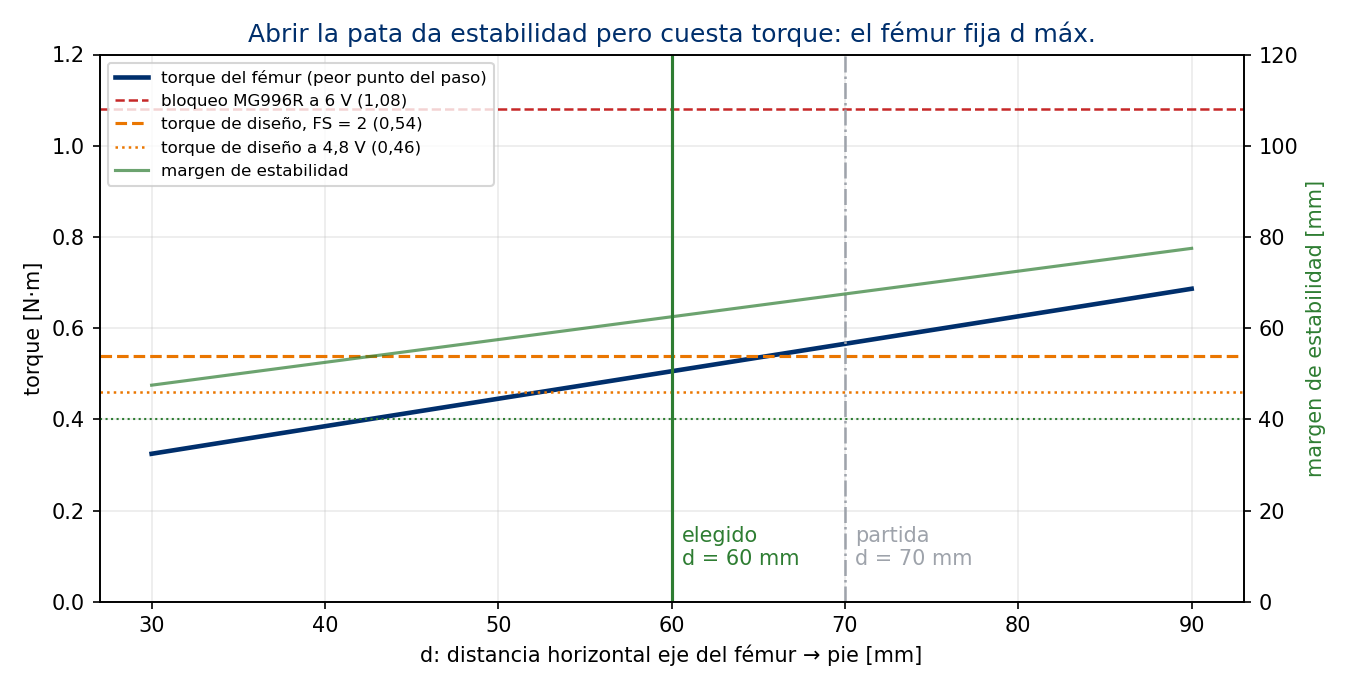
\includegraphics[width=\linewidth]{estudio_torque_vs_d.png}
\caption{Torque del fémur en el peor punto del paso y margen de estabilidad, según la distancia $d$ del eje del fémur al pie.}\label{fig:torque_d}
\end{figure}

\begin{table}[H]\centering\small
\caption{Barrido de $d$: cuántos pares $(L_2, L_3)$ cumplen y cuál está en el centro.}\label{tab:barrido}
\begin{tabular}{@{}cccccc@{}}
\toprule
$d$ [mm] & cumplen & centro $(L_2, L_3)$ & FS torque & holgura & estabilidad\\\midrule
45 & 10 & (50, 110) & 2,56 & 0,43 & 55~mm\\
50 & 20 & (60, 115) & 2,43 & 0,77 & 57~mm\\
55 & 33 & (55, 115) & 2,26 & 1,03 & 60~mm\\
\textbf{60} & \textbf{41} & \textbf{(60, 115)} & \textbf{2,14} & \textbf{1,08} & \textbf{62~mm}\\
65 & 50 & (75, 120) & 2,05 & 1,31 & 65~mm\\
70 & 12 & (105, 125) & 2,01 & 0,69 & 68~mm\\
\bottomrule
\end{tabular}
\end{table}

Se elige $d = 60$~mm: la mayor con factor de seguridad $\ge$ 2,1 (margen
para la masa real de piezas que aún no existen) y holgura $\ge$ 1 (tolera
10~mm de error).

\begin{figure}[H]\centering
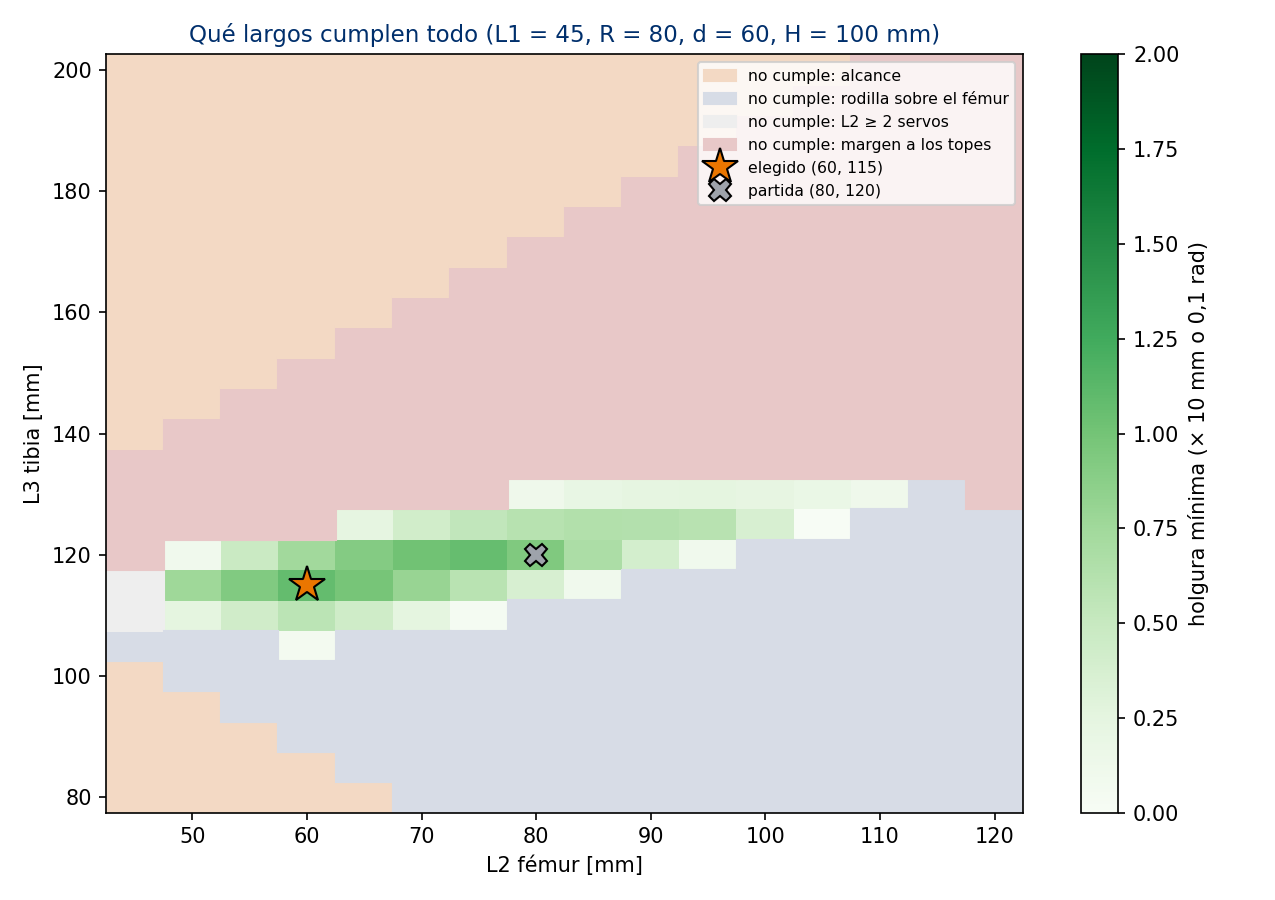
\includegraphics[width=0.9\linewidth]{estudio_mapa_largos.png}
\caption{Qué pares $(L_2, L_3)$ cumplen todo con $d = 60$~mm, y con cuánta holgura. El diseño de partida (X) estaba en el borde.}\label{fig:mapa}
\end{figure}

\subsec{Resultado}

\begin{destacado}[title=Cotas para fabricar (de eje a eje)]
\textbf{Coxa 45~mm · fémur 60~mm · tibia 115~mm · radio del cuerpo 80~mm.}
Postura de pie: pie a 60~mm del eje del fémur y 100~mm bajo el eje de la
coxa. En esta postura la tibia queda vertical (a 1°) y casi no hace torque.
\end{destacado}

\begin{figure}[H]\centering
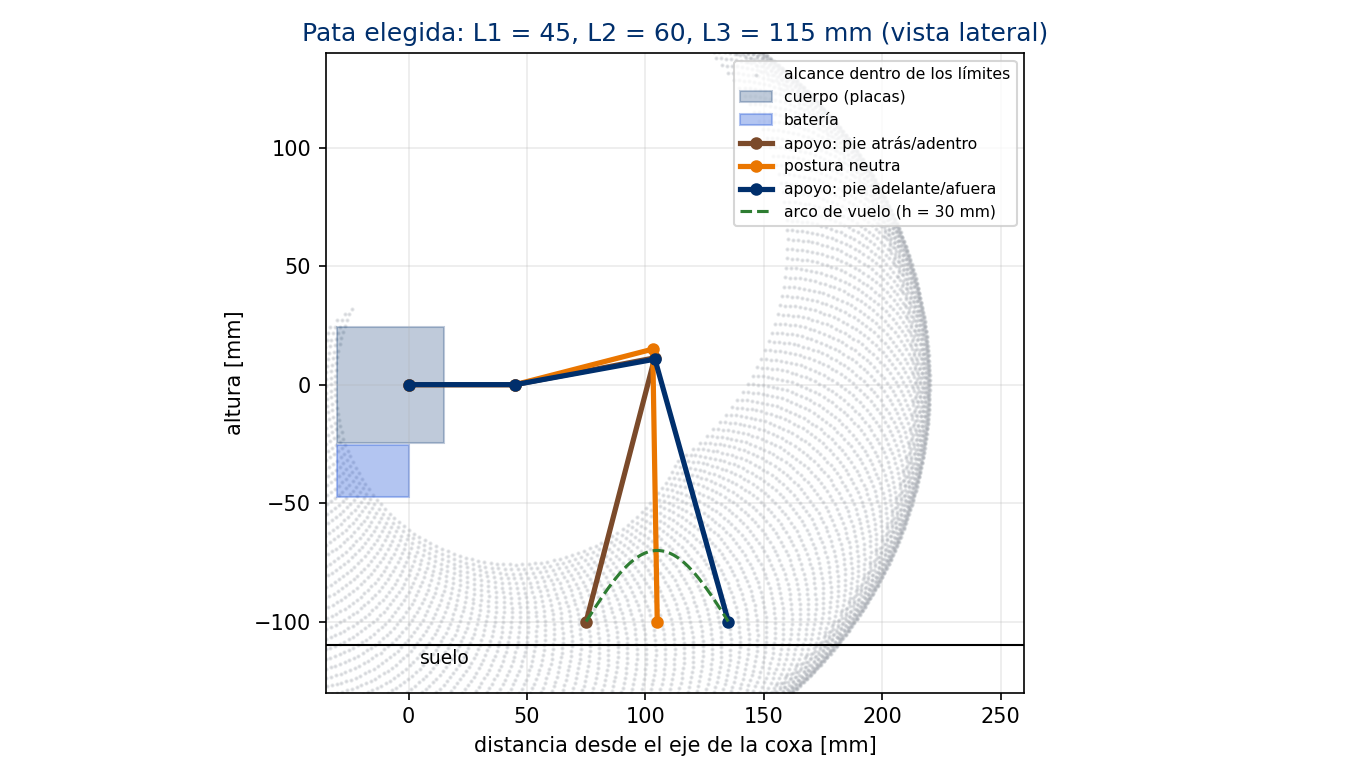
\includegraphics[width=0.95\linewidth]{estudio_pata.png}
\caption{La pata elegida de costado: postura neutra, extremos del apoyo y arco de vuelo, dentro de su espacio de trabajo.}\label{fig:pata}
\end{figure}

\begin{table}[H]\centering\small
\caption{Diseño de partida frente al diseño del estudio.}\label{tab:comparacion}
\begin{tabularx}{\linewidth}{@{}Ycc@{}}
\toprule
 & \textbf{Partida} & \textbf{Estudio}\\\midrule
$L_1$ / $L_2$ / $L_3$ & 45 / 80 / 120~mm & 45 / \textbf{60} / \textbf{115}~mm\\
Radio del cuerpo & 100~mm & \textbf{80}~mm\\
Torque del fémur, peor punto & 0,555~N·m \no & 0,506~N·m \ok\ (FS 2,14)\\
Altura libre & 52,5~mm \no & 62,5~mm \ok\\
Margen de estabilidad & 77,5~mm & 62~mm \ok\\
\bottomrule
\end{tabularx}
\end{table}

\textbf{Sensibilidad.} A 4,8~V el factor de seguridad baja a 1,82; con el
robot 200~g más pesado, a 1,91. Por eso se recomienda alimentar los servos a
6~V y respetar un presupuesto de masa de unos 1,9~kg.

\textbf{Verificación con el diseño nuevo}: de pie a 110~mm estable 60~s,
velocidad con error de 9--15\,\%, integración 8/8 y 80 tests. Un test
comprueba en cada \texttt{colcon test} que las medidas del modelo sigan
cumpliendo todas las restricciones. La especificación completa (cotas del
cuerpo, posición de cada componente y márgenes) está en
\path{docs/especificacion_diseno.md}.

%======================================================== VALIDACIÓN
\seccion{Validación e integración}

\subsec{Tests automáticos}

80 tests que se corren sin abrir Gazebo (\texttt{colcon test}):
cinemática, modelo completo (18 articulaciones, masa, centro de masa),
marcha (siempre 3 patas apoyadas, sin saltos, alcanzable a velocidad
máxima), joystick (zona muerta, curva, gradiente continuo), estudio de
dimensiones, consistencia entre el URDF y la configuración, y estilo del
código.

\subsec{Prueba de integración}

\path{scripts/prueba_integracion.py} recorre el sistema completo como un
usuario y evalúa ocho puntos con criterio numérico.

\begin{table}[H]\centering\small
\caption{Prueba de integración con el diseño final.}\label{tab:integracion}
\begin{tabularx}{\linewidth}{@{}clYc@{}}
\toprule
\# & \textbf{Prueba} & \textbf{Resultado} & \\\midrule
1 & Articulaciones publicadas & 18 & \ok\\
2 & Se para solo & 110,0~mm (± 2) & \ok\\
3 & Sensores & IMU 100~Hz, cámara 14,9~Hz & \ok\\
4 & Joystick adelante, 6~s & avanza 53~cm & \ok\\
5 & Joystick a la derecha, 5~s & gira $-107^\circ$ & \ok\\
6 & Botón + derecha, 6~s & 52~cm de lado & \ok\\
7 & Teclado atrás, 5~s & retrocede 35~cm & \ok\\
8 & Nadie publica & se detiene solo (0,0~mm en 3~s) & \ok\\
\bottomrule
\end{tabularx}
\end{table}

\subsec{Prueba en un PC limpio}

Para comprobar que el proyecto funciona en otro computador (el del
profesor), \path{scripts/prueba_en_limpio.sh} copia el último commit a
un contenedor \texttt{ros:jazzy}, que trae Ubuntu 24.04 con ROS\,2 base y
nada más, y sigue solo el inicio rápido. Ahí \texttt{./instalar.sh --test}
instaló todas las dependencias, compiló y aprobó todos los tests, y la
prueba de integración dio 8/8. El instalador usa \texttt{rosdep}, que lee
las dependencias declaradas en cada \texttt{package.xml}; por eso se
revisaron todos los \texttt{import} del proyecto contra esos archivos.

%======================================================== SUPUESTOS Y FUTURO
\seccion{Supuestos y trabajo futuro}

\subsec{Supuestos que conviene revisar}

\begin{table}[H]\centering\small
\caption{Hipótesis del modelo y qué pasa si cambian.}\label{tab:supuestos}
\begin{tabularx}{\linewidth}{@{}lYY@{}}
\toprule
\textbf{Supuesto} & \textbf{Valor} & \textbf{Si cambia}\\\midrule
Masa de la estructura & 400~g (placas y piezas de las patas) & Con 200~g más, FS 1,91: acortar $d$ o el paso\\
Cables y reguladores & 100~g & ídem\\
Torque real del servo & 1,08~N·m a 6~V (hoja) & Medir cada servo antes de montar\\
Ruido de la IMU & del orden de la hoja & Solo afecta la simulación\\
Alimentación de los servos & 6~V & A 4,8~V, FS 1,82\\
\bottomrule
\end{tabularx}
\end{table}

\subsec{Puntos por tratar}

\begin{itemize}
  \item \textbf{Prueba del joystick con la placa} (D17): todo está listo; se
  hace al comprar la ESP32 siguiendo \path{docs/joystick_esp32.md}.
  \item \textbf{Pequeño retroceso al detenerse}: al soltar el mando el cuerpo
  frena en unos 0,4~s, pero mientras los pies vuelven a su posición neutra
  puede retroceder entre 1 y 24~mm según el momento del paso. Mejora
  posible: volver a casa más lento o solo con los pies que quedaron lejos.
  \item \textbf{Torque caminando}: el simulador no entrega la carga dinámica
  real (ver «Marcha trípode»). Una mejora sería modelar el servo con control de
  torque (fuerza proporcional al error, como un servo real).
\end{itemize}

\subsec{Hacia el robot real}

\begin{enumerate}
  \item Fabricar las piezas con las cotas del estudio y pesarlas; poner las
  masas reales en \texttt{hexapod\_params.xacro} y volver a correr el estudio.
  \item Alimentar los servos a 6~V con reguladores (UBEC) de 10--20~A y un
  fusible en la LiPo.
  \item Escribir el driver de \texttt{ros2\_control} para las PCA9685: el
  resto del software no cambia.
  \item Conectar la BNO085 por SPI o UART (tiene problemas conocidos con el
  I2C de la Raspberry).
\end{enumerate}

%======================================================== CONCLUSIONES
\seccion{Conclusiones}

\begin{enumerate}
  \item Se cumplió la pauta de la Evaluación~1 con un robot más complejo que
  el pedido: 18 articulaciones, base flotante y marcha, con todo verificado
  por mediciones y no solo por inspección visual.
  \item La simulación sirvió para algo más que mostrar: \textbf{encontró dos
  fallas del diseño de partida} (sobrecarga del fémur y poca altura libre)
  antes de fabricar una sola pieza, y entregó cotas con su justificación.
  \item Separar la lógica de ROS y medir con scripts permitió detectar y
  explicar efectos del simulador (el torque caminando) en vez de tomarlos
  como ciertos.
  \item El proyecto es reproducible: un comando lo instala y una prueba en un
  PC limpio lo confirma.
\end{enumerate}

%======================================================== GLOSARIO
\seccion{Glosario}

\begin{tabularx}{\linewidth}{@{}lY@{}}
\toprule
\textbf{Término} & \textbf{Significado}\\\midrule
Coxa, fémur, tibia & Los 3 segmentos de la pata, del cuerpo al pie\\
$L_1, L_2, L_3$ & Largos de coxa, fémur y tibia, de eje a eje\\
FK / IK & Cinemática directa (ángulos → posición) e inversa (posición → ángulos)\\
Marcha trípode & Dos grupos de 3 patas que se alternan\\
$\beta$, $T$, $\Delta$ & Fracción del ciclo en apoyo, duración del ciclo, vector de paso\\
Base flotante & El cuerpo no está unido al mundo; se sostiene con los pies\\
Factor de seguridad (FS) & Torque de bloqueo dividido por el torque que se exige\\
URDF / xacro & Descripción del robot en XML / con variables y macros\\
TF & Sistema de marcos de coordenadas de ROS\\
REP-103 & Convención de ROS: $x$ adelante, $y$ izquierda, $z$ arriba; unidades SI\\
\texttt{ros2\_control} & Estándar de ROS para controlar articulaciones\\
Puente (\emph{bridge}) & Traductor de tópicos entre Gazebo y ROS\\
micro-ROS / agente & ROS para microcontroladores / programa del PC que lo conecta\\
Zona muerta / expo & Rango central de la palanca que vale 0 / curva que afina el centro\\
\texttt{rosdep} / \texttt{colcon} & Instalador de dependencias / compilador del workspace\\
\bottomrule
\end{tabularx}

%======================================================== REFERENCIAS
\Needspace{14\baselineskip}
\addcontentsline{toc}{section}{Referencias}
\begin{thebibliography}{99}\small
\bibitem{ros2} Open Robotics. \emph{ROS\,2 Documentation: Jazzy}. \url{https://docs.ros.org/en/jazzy/}
\bibitem{rep103} T.~Foote, M.~Purvis. \emph{REP 103: Standard Units of Measure and Coordinate Conventions}. \url{https://reps.openrobotics.org/rep-0103/}
\bibitem{ros2control} ros2\_control. \emph{Documentación (Jazzy)}. \url{https://control.ros.org/jazzy/}
\bibitem{gzros2control} ros2\_control. \emph{gz\_ros2\_control}. \url{https://control.ros.org/jazzy/doc/gz_ros2_control/doc/index.html}
\bibitem{gazebo} Open Robotics. \emph{Gazebo Harmonic}. \url{https://gazebosim.org/docs/harmonic/}
\bibitem{rosgz} Gazebo. \emph{ros\_gz: integración ROS\,2 – Gazebo}. \url{https://github.com/gazebosim/ros_gz}
\bibitem{microros} micro-ROS. \url{https://micro.ros.org/}
\bibitem{microrospio} micro-ROS. \emph{micro\_ros\_platformio}. \url{https://github.com/micro-ROS/micro_ros_platformio}
\bibitem{mg996r} Tower Pro. \emph{MG996R High Torque Metal Gear Servo} (hoja de datos, copia de Cornell ECE). \url{https://people.ece.cornell.edu/land/courses/ece4760/FinalProjects/f2017/kmv48_rp625/kmv48_rp625/kmv48_rp625/MG996RTowerPro.pdf}
\bibitem{bno085} Adafruit. \emph{9-DOF Orientation IMU Fusion Breakout -- BNO085}. \url{https://learn.adafruit.com/adafruit-9-dof-orientation-imu-fusion-breakout-bno085}
\bibitem{picam3} Raspberry Pi Ltd. \emph{Camera Module 3}. \url{https://www.raspberrypi.com/documentation/accessories/camera-module-3.html}
\bibitem{wilson1966} D.~M.~Wilson (1966). Insect walking. \emph{Annual Review of Entomology}, 11, 103--122.
\end{thebibliography}

\end{document}
